\documentclass{article}

% Import Packages =======================================
\usepackage[parfill]{parskip}
\usepackage{listings}
\usepackage{xcolor}
\usepackage{hyperref}
\usepackage{url}
\usepackage{floatrow}
\usepackage{multirow}
\usepackage{multicol}
\usepackage{graphicx}

\usepackage{amsmath}
\usepackage{amsthm}
\usepackage{amssymb}
\usepackage{esint}

% Set lstlistings ========================================
\lstset{
    numbers=left,
    language=[LaTeX]TeX,
    breaklines=true,
    keywordstyle=\color{blue}\bfseries,
    numberstyle=\tiny\color{gray},
    commentstyle=\color{green!30!black},
    stringstyle=\color{violet},
}

\lstnewenvironment{TeXlstlisting}{\lstset{language=[LaTeX]TeX}}{}

% Theorem Environments ==================================
\newtheorem{theorem}{Theorem}
\newtheorem{lemma}{Lemma}
\newtheorem{proposition}{Proposition}[section]

\theoremstyle{remark}
\newtheorem*{remark}{Remark}
\newtheorem*{hint}{Hint}

% Code Environment ======================================
\newcounter{listing}

\newenvironment{code}[2]
% Argument 1 = Language
% Argument 2 = Text below heading
{
    \begin{center}
        \refstepcounter{listing}
        \textbf{\large Listing \thelisting: #1} \\
        \textbf{#2}
    \end{center}
}
{
    \vspace{2em}
}

% Make Title
\title{Technical Typesetting Assignment} 
\author{Prakhar Mittal}
\date{15 July 2020}


% Begin Document =========================================
\begin{document}
    
\maketitle
\tableofcontents

\newpage

\section{Listings and Environments}

\begin{code}{[LaTeX]TeX}{An Example}

\begin{TeXlstlisting}
\begin{lstlisting}
% A regular \lstlisting environment won't work. You'll have to use \lstnewenvironment to define a custom environment.
\end{lstlisting}
\end{TeXlstlisting}

\end{code}

\begin{code}{Python}{Regular Stuff}

\begin{lstlisting}[language=python]
from scipy import *
#The custom environment you define should be numbered as well. We did this in our tutorial. Think about what arguments you can pass to it.
print("Hello!")
\end{lstlisting}

\end{code}

\begin{code}{C++}{Generic Title}

\begin{lstlisting}[language=c++]
#include <iostream>
using namespace std;

//From the three examples, you must have observed what you can hardcode.


int main(int argc, char* argv[])
{
    cour<<"Hello!"<<endl;
}
\end{lstlisting}

\end{code}
The \verb!2em! vertical space aafter the listing is part of the custom environment.

\newpage

\section{Formal Logic: Figures and Tables}

\begin{figure}[H]
    \centering
    \begin{floatrow}
        \ffigbox[0.4\textwidth]{\caption{Aristotle: the first formal logician}}{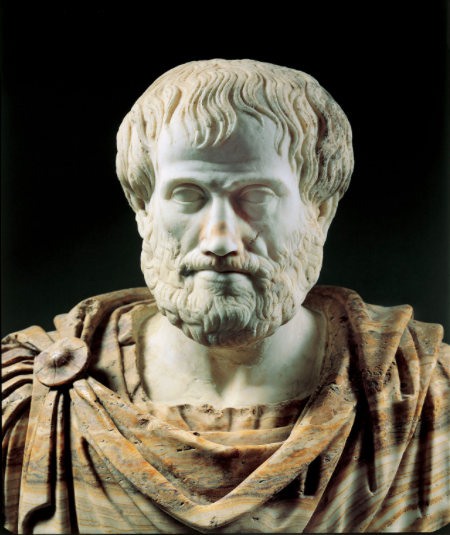
\includegraphics[width=0.4\textwidth]{aristotle.png}}
        \ffigbox[0.5\textwidth]{\caption{Saul Kripke: we've come a long way since then.}}{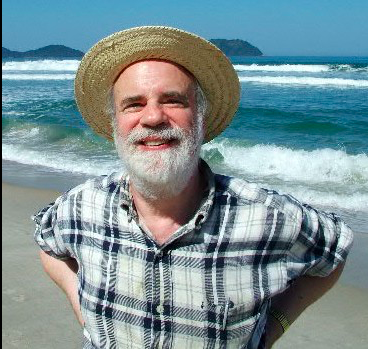
\includegraphics[width=0.5\textwidth]{kripke.png}}
    \end{floatrow}
    \label{philosophers}
\end{figure}

\href{https://www.britannica.com/biography/Aristotle#/media/1/34560/76426}{Aristotle image source} \\
\href{https://commons.wikimedia.org/w/index.php?curid=5763037}{Saul Kripke image source} \\
Make sure you follow these links, so you know where the hyperlinks lead to when you typeset it yourself.

\begin{table}[H]
    \centering
    \begin{tabular}{lcccc|lcccc}
        \hline
        \textbf{Assertion}& & & & & \textbf{Negation} & & & & \\
        \hline
        \multicolumn{5}{l|}{$p(x)$} & \multicolumn{5}{l}{$\neg p(x)$} \\
        \hline
        \multicolumn{5}{l|}{\multirow{2}{*}{$\perp$}} & \multicolumn{5}{l}{$p(x) \vee \neg p(x)$} \\
        & & & & & $\top$ & & & & \\
        \hline
        \multicolumn{5}{l|}{\multirow{2}{*}{$p(x) \wedge q(x) $}} & \multicolumn{5}{l}{$\neg(p(x) \wedge q(x))$} \\
        & & & & & \multicolumn{5}{l}{$\neg p(x) \wedge \neg q(x)$} \\
        \hline
        \multicolumn{5}{l|}{$\exists x.p(x)$} & \multicolumn{5}{l}{$\forall x.\neg p(x)$} \\
        \hline
        \multicolumn{5}{l|}{\multirow{2}{*}{$p(x) \Rightarrow q(x) $}} & \multicolumn{5}{l}{$\neg(\neg p(x) \vee q(x))$} \\
        & & & & & \multicolumn{5}{l}{$p(x) \wedge \neg q(x)$} \\
        \hline
        \multicolumn{10}{c}{This statement is false} \\
        \hline
    \end{tabular}
    \caption{Some First Order Logic, and an absurdity.}
\end{table}

This table uses \verb!multirow! as well as \verb!multicolumn!. Replicate it as well as you can.

\clearpage

\section{Maths, Theorems and References}

\begin{theorem}[Divergence Theorem]
    \begin{equation*}
        \iiint_V(\boldsymbol{\nabla~\cdot}~\mathbf{F})dV = \oiint_S(\mathbf{F}\cdot \mathbf{\hat n})dS
    \end{equation*}
\end{theorem}

\begin{remark}
    You have efinitely studied and applied the theorem extensively in MA 105. It 
    also showls up as Gauss's Law in electrodynamics.
\end{remark}

\begin{proposition}[Georg Cantor]
    Let $\mathbb{N}$ be the set of natural numbers. Denoe its cardinality $|\mathbb{N}|$ by $\aleph _0$. Let 
    $\mathbb{R}$ be the set of real numbers. Its cardinality $\mathfrak{c}$ is sometimes called the cardinality
    of the continuum. $\mathfrak{c}=2^{\aleph_0}$
\end{proposition}

\begin{hint}
    You will find the \verb!\mathfrak! command useful to typeset the above.
\end{hint}

\begin{lemma}[Jordan Normal Form]
    \label{lemma}
    For every matrix M in $\mathbb{C}^{\kappa \times \kappa}$ having eigenvalues $\gamma_1$,\dots,$\gamma_k$,
    with algebraic multiplicities $m_1,\dots,m_k$ respectively, there is an invertible matrix
    P and a matrix D of the form D = Diag($J_1,\dots,J_k$) with each block $J_i$ being a $m_i \times m_i$ matrix of the form

    \begin{equation*}
        J_i = \begin{bmatrix}
            \gamma_i & 1 & 0 & \dots & 0 \\
            0 & \gamma_i & 1 & \dots & 0 \\
            \vdots & \vdots & \vdots & \ddots & \vdots \\
            0 & 0 & 0 & \dots & 1 \\
            0 & 0 & 0 & \dots & \gamma_i
        \end{bmatrix}
    \end{equation*}
    and $M=P^{-1}DP$. Moreover, if M is an algebraic matrix, so are D and P, and 
    their entries can be computed from the entries of $M$.
\end{lemma}
    
You have certainly studied that if $M$ is defect free, that is, algebraic and multiplicities
of its eigenvalues coincide, then it is similar to a diagonal matrix. If not,
the Jordan Normal form is the next best thing. We cite \cite{linalg} for this lemma.

\begin{hint}
    Look at the bibliography entry for this citation. It is a book. Specify the author,
    publisher, title, year and edition. Our bibliography style is \verb!plainurl!
\end{hint}

Consider the last statement of Lemma \ref{lemma}. (Yes, a cross reference.) Algebraic numbers
are roots of polynomials with integer coefficients. They can be found efficiently.\cite{cite2}

\begin{hint}
    This citation is and article. Specify the author, year, title, journal, volume and number.
\end{hint}

\bibliographystyle{plainurl}
\bibliography{190070046_3}

\end{document}